%=========================================================================
% (c) 2014, 2015 Josef Lusticky

\section{Software}

To perform the measurements, base CentOS 7 was installed on the server.
The operating system features Linux kernel based on version 3.10 -
the installed version was 3.10.0-123.20.1.el7.x86\_64.
The system detects the Mellanox ConnectX-3 EN card automatically and loads the mlx4\_core and mlx4\_en module.
The mlx4\_core module prints the detected PCI-Express link parameters to the message buffer of the kernel.
This buffer can be viewed using the dmesg command and it is shown bellow:
\begin{lstlisting}[language=TeX]
mlx4_core 0000:06:00.0: PCIe link speed is 8.0GT/s, device supports 8.0GT/s
mlx4_core 0000:06:00.0: PCIe link width is x8, device supports x8
\end{lstlisting}
The mlx4\_core module further registers interrupts and prints the assigned IRQ numbers for each queue
to the message buffer of the kernel:
\begin{lstlisting}[language=TeX]
mlx4_core 0000:06:00.0: irq 61 for MSI/MSI-X
mlx4_core 0000:06:00.0: irq 62 for MSI/MSI-X
...
mlx4_core 0000:06:00.0: irq 90 for MSI/MSI-X
\end{lstlisting}

The driver uses MSI or MSI-X feature of the PCI-Express bus, as described in section~\ref{sec:40gbe-throughput}.
The MSI-X feature is used automatically if the system supports it, otherwise the adapter uses MSI.
The lspci -vv command can be used to check whether MSI-X is used.
The MSI-X capability is followed by an Enable flag which is followed with either "+" (enabled)
or "-" (disabled).
Listing~\ref{lst:setup-lspci} shows part of its output for the Mellanox ConnectX-3 EN adapter.
\begin{lstlisting}[language=TeX,label={lst:setup-lspci},caption={Partial output of lspci -vv for Mellanox ConnectX-3 EN}]
06:00.0 Ethernet controller: Mellanox Technologies MT27500 Family [ConnectX-3]
		...
		Capabilities: [9c] MSI-X: Enable+ Count=128 Masked-
				...
				LnkCap: Port #8, Speed 8GT/s, Width x8, ASPM L0s, Exit Latency L0s unlimited, L1 unlimited
				...
\end{lstlisting}



Apart from the NIC driver, which is part of kernel package, the Mellanox ConnectX-3 adpater uses its own firmware.
The firmware can be updated using the Mellanox Firmware Tools (MFT), which can be downloaded
from the Mellanox management tools site.\footnote{{\url{http://www.mellanox.com/page/management_tools}}}
Installation of Mellanox Firmware Tools is described in MTF User Manual available at
the Mellanox documentation site.\footnote{{\url{http://www.mellanox.com/related-docs/MFT/MFT_user_manual.pdf}}}
The installation consists of unpacking the downloaded MFT archive and running the {\it{install.sh}} script.
This will install kernel-mft and mft packages.
The kernel-mft package contains required low-level kernel drivers, whereas the mft package contains utilities which use these drivers.
To start the Mellanox Software Tools service, which also loads the kernel drivers, run {\it{mst start}}.
Afterwards, the utilities from the mft package can be used, including the mlxfwmanager for updating the firmware.
The mlxfwmanager displays various information about the adapter, including the firmware version.

The newest firmware for the Mellanox ConnectX-3 adapters can be downloaded
from the Mellanox firmware site.\footnote{{\url{http://www.mellanox.com/page/firmware_table_ConnectX3EN}}}
Unzip the firmware and use the {\it{mlxfwmanager -u}} command in the same directory where the firmware was unzipped.
This will update the firmware.
After the update is complete, reboot is required to take effect.

Listing~\ref{lst:setup-firmware-update} shows the output of the firmware update procedure using the {\it{mlxfwmanager -u}} command.
The current firmware version is 2.31.5050, whereas the newer firmware placed in the current working directory is of version 2.32.5100.
The mlxfwmanager\_pci utility can be used to query the adpater information without starting the mst service.
\begin{lstlisting}[language=TeX,label={lst:setup-firmware-update}]
[root@server]# mlxfwmanager -u
Querying Mellanox devices firmware ...

Device #1:
----------

  Device Type:      ConnectX3
  Part Number:      MCX314A-BCB_Ax
  Description:      ConnectX-3 EN network interface card; 40GigE; dual-port QSFP; PCIe3.0 x8 8GT/s; RoHS R6
  PSID:             MT_1090110023
  PCI Device Name:  /dev/mst/mt4099_pci_cr0
  Port1 MAC:        f452145e6c70
  Port2 MAC:        f452145e6c71
  Versions:         Current        Available     
     FW             2.31.5050      2.32.5100     
     PXE            3.4.0225       3.4.0306      

  Status:           Update required

---------
Found 1 device(s) requiring firmware update...

Perform FW update? [y/N]: y
Device #1: Updating FW ... Done

Restart needed for updates to take effect.
\end{lstlisting}

%By default, the driver uses adaptive interrupt moderation for the receive path,
%which adjusts the moderation time to the traffic pattern~\cite{mellanox-user-manual}.




\section{Generating 40 Gigabit traffic}
%Thus the maximum effeciency of Ethernet is while transmitting the maximum sized frames.
% - selecting packet generator and how to measure
Generating 40 Gigabit traffic is not an easy task.
Basically, there are two choices how to generate such a traffic.
Either by using traditional software packet generator,
limited by the CPU speed and the optimisation level of the software,
or use a specialised hardware packet generator.

Software packet generators:
the most known pktgen,
netmap with VALE framework.

Spirent Communications is a hardware packet generator vendor,
oriented in network testing for enterprises and data centres. % TODO ~\cite{spirent}.
Among their products, a hardware packet generator called Spirent % TODO
can be found.



78 = 40 IPv6 + 20 UDP + 18 Ethernet
20~Bytes for UDP, 20 is TCP header, UDP with no data..


\begin{figure}
	\centering
	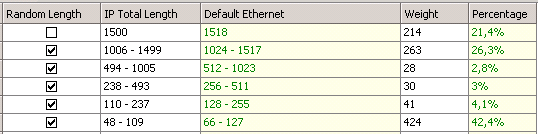
\includegraphics[width=14.5cm,keepaspectratio]{fig/amsix-imix.png}
	\caption{AMS-IX iMix}
	\label{fig:setup-amsix-imix}
\end{figure}


\section{Collecting statistics}
Per interface statistics are provided by the kernel via {\it{/proc/net/dev}} file.
This file provides statistics such as bytes received or transmitted, number of packets, errors, etc.
It is also used by the {\it{ifconfig}} utility.

Each device driver provides individual statistics for the corresponding interfaces it manages through
files found under {\it{/sys/class/net/IFNAME/statistics/}}.

The CPU utilisation can be observed in real-time by the {\it{top}} utility.
The {\it{mpstat}} utility, which is reports various processors related statistics,
did not provide accurate CPU utilisation in experiments.


Intel Performance Counter Monitor (PCM)~\footnote{https://software.intel.com/en-us/articles/intel-performance-counter-monitor-a-better-way-to-measure-cpu-utilization}
Non-maskable interrupt watchdog must be disabled
in order to run Intel PCM.
echo 0 > /proc/sys/kernel/nmi\_watchdog
